%%
%% This is file `thesis-ex.tex',
%% generated with the docstrip utility.
%%
%% The original source files were:
%%
%% uiucthesis2009.dtx  (with options: `example')
%% 
\def\fileversion{v2.25a} \def\filedate{2009/10/10}
%% Package and Class "uiucthesis2009" for use with LaTeX2e.
\documentclass[edeposit,10pt,fullpage]{uiucthesis2009}

\usepackage{amsmath, amsthm, amssymb}
\usepackage[numbers]{natbib}

\usepackage{color}
\usepackage{verbatim}

\usepackage{subfigure}
\usepackage{url}
\usepackage{times}
\usepackage{mathptmx}
\usepackage[ruled,vlined]{algorithm2e}
\usepackage[pdftex]{graphicx}
\usepackage{booktabs}

\usepackage{subfigure}
\usepackage{caption}
\usepackage{tikz}
\usetikzlibrary{arrows,positioning,fit,scopes}
\usetikzlibrary{shapes.multipart}

\colorlet{d}{black!25}
\colorlet{l}{black!0}
\newcommand{\btnode}[4]{ \nodepart{#1} #2\\ $[$#3,#4) }
\newcommand{\btplainnode}[2]{ \nodepart{#1} #2  \\  }
\tikzset{nd/.style={rectangle split, rectangle split parts=3, draw=black!75, thick,
            rectangle split horizontal, align=center, rectangle split empty part width=0.5cm,
            rectangle split part fill={#1}}}

\usepackage[pdfborder={0 0 0}]{hyperref}

\interfootnotelinepenalty=10000  % Split footnote are annoying

\newcommand{\ntaskip}{\vspace{-0.15in}}
\SetAlgoSkip{ntaskip}

\newenvironment{captiontext}{%
   \begin{center}%
     \begin{minipage}{0.99\linewidth}%
       \renewcommand{\baselinestretch}{0.9}%
         \sffamily\footnotesize}%
   {\renewcommand{\baselinestretch}{1.0}%
      \end{minipage}%
        \end{center}}

\newenvironment{smitemize}%
  {\begin{list}{$\bullet$}%
     {\setlength{\parsep}{0pt}%
      \setlength{\topsep}{0pt}%
      \setlength{\itemsep}{2pt}}}%
  {\end{list}}

\clubpenalty=10000  % Don't allow orphans
\widowpenalty=10000 % Don't allow widows

% \raggedbottom

\renewcommand{\textfraction}{0}
\renewcommand{\topfraction}{1}
\renewcommand{\bottomfraction}{1}
\setcounter{totalnumber}{10}
\setcounter{topnumber}{10}
\setcounter{bottomnumber}{10}
\setcounter{dbltopnumber}{10}
\renewcommand{\floatpagefraction}{1}
\renewcommand{\dblfloatpagefraction}{1}

%Remove this at the end.
\newcommand{\citetemp}[1]{(#1)}
\newcommand{\temp}[1]{?#1?}

\begin{document}

\title{System and Framework for Identification of Info Malware on the Android Operating System}
\author{Robert Marsan}
\department{Computer Science}
\schools{M.S, University of Illinois at Urbana-Champaign, 2013}
\msthesis
\advisor{Roy H. Campbell}
\degreeyear{2013}
\committee{Professor Roy H. Campbell}
\maketitle

\frontmatter

%% Create an abstract that can also be used for the ProQuest abstract.
%% Note that ProQuest truncates their abstracts at 350 words.
\begin{abstract}
The tremendous rise of mobile computing has led to an equally strong rise in mobile malware. We address this issue with several novel concepts, permission fingerprints and user-app agreements. We also present a groundbreaking and substantial new dataset of the state of Android Apps, and provide unique results gathered from it. Finally, we present AndroMEDA, an Android Security Extension which helps address many of the shortcomings to existing techniques of malware identification currently available.


This $seriously$ needs to be extended.

\end{abstract}

%% Create a dedication in italics with no heading, centered vertically
%% on the page.
\begin{dedication}
To my\\
Parents, Lisa and Mark
\end{dedication}

%% Create an Acknowledgements page, many departments require you to
%% include funding support in this.
\chapter*{Acknowledgments}

I would like to thank my advisor Roy H. Campbell for his mentorship and guidance, as well as Alejandro Gutierrez for putting up with me.

%% The thesis format requires the Table of Contents to come
%% before any other major sections, all of these sections after
%% the Table of Contents must be listed therein (i.e., use \chapter,
%% not \chapter*).  Common sections to have between the Table of
%% Contents and the main text are:
%%
%% List of Tables
%% List of Figures
%% List Symbols and/or Abbreviations
%% etc.

\tableofcontents
\listoftables
\listoffigures
\listofalgorithms

%this can add another section...?
%\addcontentsline{toc}{chapter}{List of Algorithms}

%% Create a List of Abbreviations. The left column
%% is 1 inch wide and left-justified
%\chapter{List of Abbreviations}
%
%\begin{symbollist*}
%\item[CA] Caffeine Addict.
%\item[CD] Coffee Drinker.
%\end{symbollist*}

%% Create a List of Symbols. The left column
%% is 0.7 inch wide and centered
%\chapter{List of Symbols}

%\begin{symbollist}[0.7in]
%\item[$\tau$] Time taken to drink one cup of coffee.
%\item[$\mu$g] Micrograms (of caffeine, generally).
%\end{symbollist}

\mainmatter
\chapter{Introduction}
\label{sec:intro}

%\textbf{Thesis Statement}: Malware, and especially Info Theft Malware, on Mobile Operating Systems, especially Android, is better understood when not just analyzing the capabilities of an application, but the expectations the user has as to how it utilizes those capabilities as well.\\
%\textbf{Thesis Statement}: Android Malware detection is complemented by not just analyzing the capabilities of an app, but the context and use as well.\\
%\textbf{Thesis Statement}: In order to detect Android Malware, the user must understand what is going on behind the scenes of the app. The capabilities of an app are important, but the context and use of these capabilities are as well.\\
\textbf{Thesis Statement}: Using a novel feedback loop, we provide users with a method for understanding the context and use of actions an app performs, thus allowing them to identify suspicious behavior that violates users' trust.\\


The rise of smartphones in the last decade years has been unprecedented. Since the launch of the Apple iPhone in 2007, there are now almost 1 Billion smartphone users in the world\citep{kpcbinternetreport2012}. These new devices marked an unprecedented shift in our relationship with computers, becoming the center point for many personal endeavors, and superseding almost all previous computing devices from cell phones, to cameras, to GPS devices, and to most uses of a desktop PC\citep{hua2012introduction}. Smartphones continue to become the focal point of almost all personal computing, and consequently the operating systems they run become more important and powerful.

\section{Contributions}
In this thesis, we highlight 4 key areas:
\begin{smitemize}
\item \textit{User-App Agreement}: First, we discuss the challenges of addressing modern mobile malware, and the shortcomings of the Android security model. We introduce the User-App Agreement (UAA), a way of conceptualizing the trust a user has in actions an applications may perform, as a key component in identifying malicious behavior.
\item \textit{Android Census}: Second, we use a novel dataset, Android Census, to examine the state of Android permissions. We find Android permissions correlate with expected use, but key examples are shown of less than legitimate use. Using a comprehensive set of malware, we cross examine how the permissions of malware compares with the Android Census. We conclude that malware that targets the user's personal information is the most difficult to detect using this static analysis.
\item \textit{IncognitoWare}: Third, we address the shortcomings of the current malware datasets available to academia, and introduce a new dataset of IncognitoWare. This dataset is more representative of current trends in malware, and proves to be a great challenge to detect.
\item \textit{AndroMEDA}: Finally, we introduce Android Malware Evaluation Detection and Analysis (AndroMEDA), a set of Android extensions, and a companion app, build off of the premise of the User-App Agreement. By giving the user more information on the context and use of sensitive system actions, they can evaluate whether they trust those actions, and ultimately whether the app is acting maliciously or not.
\end{smitemize}
\subsection{}





% After untrusted behavior is spotted, the actions can be reported, and knowledge can be spread to all users. All of this makes users more aware of app behavior, and helps mitigate Info Theft Malware on Android.

%Building off the concept of the User-App Agreement, we introduce AndroMEDA. Key parts of the User-App Agreement were previously unnoticable to the user until AndroMEDA. By giving the user more information on the context and use of permissions, they can evaluate whether they trust those actions, and ultimately whether the app is acting maliciously or not. After untrusted behavior is spotted, the actions can be reported, and knowledge can be spread to all users. All of this makes users more aware of app behavior, and helps mitigate Info Theft Malware on Android.


%This security model has dramatically changed the nature of mobile software, and in turn, mobile malware. By forcing malware to fit inside of this security sandbox, malware authors must choose to either break out of the box, or work inside of it. This constriction has blurred the definition of mobile malware, and ultimately has profound implications for the user of the mobile device. We will examine these implications, and propose new tools and methods to help understand the nuances of modern malware, as well as provide a framework of tools to detect them.


\chapter{Background \& Motivation}
\label{sec:background}

%To understand the nature of modern mobile malware, we first examine the context. The two main models, that of iOS and Android, are compared and contrasted here.

\section{The ``App'' and Sandboxing}

In the mobile world, ``Apps'' are isolated and sandboxed programs, generally designed with one singular purpose. They lack dependencies, and generally are not as privileges as system software for performing many tasks. The mechanisms for accessing functionality outside of their sandbox is enforced by a set of policies the system holds, specific to that app. On some platforms, like iOS, only one app may run at any given time, and background computation is virtually non-existent (with some exceptions)\footnote{Minor amounts of computation can be done to compute background audio, and other isolated background tasks.}, along with many other restrictions. On Android and other platforms, many more features are available to apps, but in all cases, the ``app'' lifecycle is well defined and controlled by the system much more than on a PC OS.

There are various reasons for the tight sandboxing of mobile apps. Power and resource consumption are certainly a factor - mobile OSs generally reserve the right to kill apps if they attempt to allocate too much memory. Controlling access to hardware also helps in this: allowing apps to keep the phone awake could easily drain battery. However, another reason for sandboxing, and arguably more important, is protecting Personally Identifiable Information.

\subsection{Personally Identifiable Information}

Personally Identifiable Information (PII), as defined by the National Institute of Standards and Technology, is ``any information about an individual maintained by an agency, including (1) any information that can be used to distinguish or trace an individual‘s identity... and (2) any other information that is linked or linkable to an individual'' \citep{mccallister2010guide}. Mobile devices, having blended cameras, cell phones, GPS devices, and PCs into one device, have an extremely diverse amount of PII, from phone numbers, to contacts, to location history, to bank account numbers and pictures. For many of these datasets, mobile OSs actually organize them into databases with the intention of allowing 3rd parties access to them. Contact lists, SMS, Photographs and location history are available to apps on virtually every mobile platform in some official way. This is a driving motivation for a greatly improved security model for mobile OSs: controlling 3rd party software's access to PII. 

% Expand more on this.

\subsection{Digital Distribution Platform}

The final major difference between mobile OSs and PC OSs is the distribution of code. No mobile OS allows 3rd party code to be ran outside of the sandbox, and all of them require the user's consent before installing an app. All apps must be signed, and in general, there is 1 main distribution channel for all apps on a mobile OS. This tightly controlled distribution both aids in security, as well as controls the ecosystem around that mobile OS.

\subsection{Apple's App Store}
The first major digital distribution platform for mobile apps was Apple's App Store\citep{AppleAppStore}. It's model has been repeated by almost all major mobile app distribution platforms. The basic premise is simple: developers sign up to the app store, pay a fee (usually yearly), and submit fully-finished apps. A reviewer runs the app in a monitored sandbox, watches for unusual behavior, checks for stability and usability, and approves it. Once the app has been approved, it's released onto the app store, at which time anyone can download it. The approval process, as well as the high monetary fee, act as a way to ensure only safe and high-quality apps are available for that platform. In this type of platform, typically no apps may be installed from other sources. On iOS, initially this was the main method of security: if the app passed the inspection, it was acknowledged as safe and virtually unmonitored unless someone noticed something unusual and reported it. However, in recent years, after certain incidents (see section \ref{sec:path}), apps still must request permission from the user to perform certain tasks.

\subsection{Android Permissions}
Android's distribution platform takes a different approach, and at it's core is also Android's security model: The Permission System (see section \ref{sec:permissions}). Android Apps declare when they are packaged what capabilities they will use, and the user reviews them at install time. If the user approves the app, it may use the requested capabilities whenever it wants: little restrictions are placed otherwise. With this barrier in mind, the Google Play Store (formerly known as the Android Market), or GPStore, opts for an alternate model to iOS, where the developer pays a smaller fee, and apps go through no formal approval process. After an app's submission, it's immediately released into the wild for users to download and run. The assumption Android uses is that the metadata the GPStore provides: App name, Developer Name, Description, Reviews and Ratings, are enough for the user to determine if the app should be trusted with the permission set it's given (see Figure \ref{fig:gpstoreapps}). In fact, Android even allows the device to accept apps from 3rd party sources, a practice known as ``sideloading'', although it's disabled by default. This has spawned a large number of 3rd party app sources, all of which rely on the Permission system for user protection.

%GPSTORE IMAGE AND CHART EXPLAINING THE LETTERS.

\begin{figure}[h]
\begin{center}
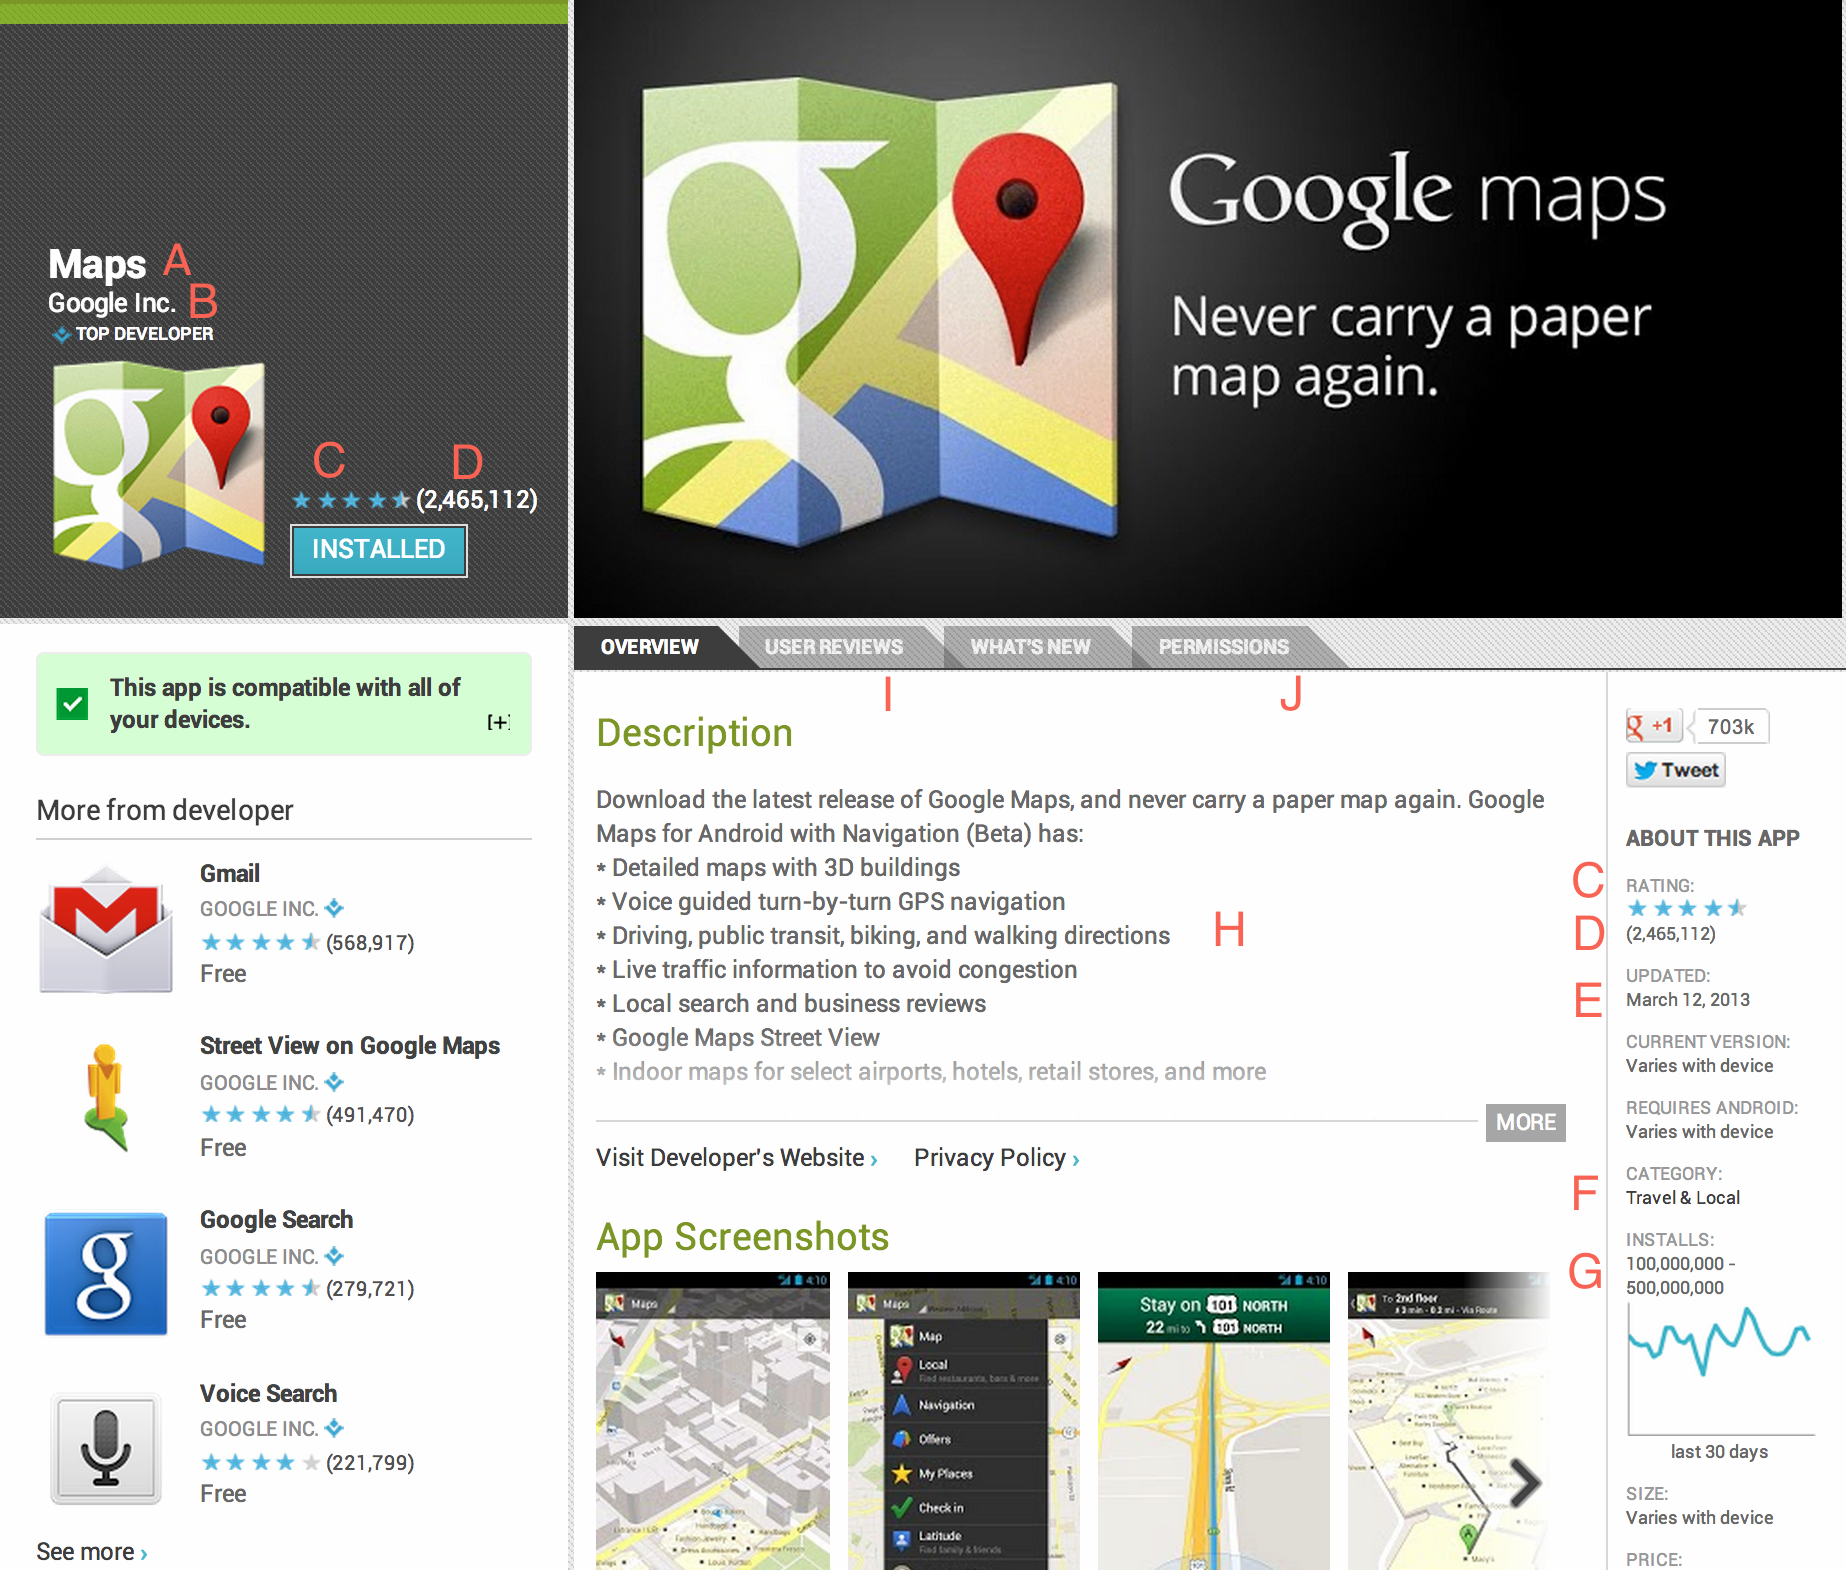
\includegraphics[width=0.9\columnwidth]{figs/GPStoreAppPage}
\caption{A sample page on the Google Play Store, see \ref{tab:gpstorekey}}
\label{fig:gpstoreapps}
\end{center}
\end{figure}

\begin{table*}[h]
\begin{small}
\begin{tabular}{l|l}

\textit{A} & App name  \\
\textit{B} & Developer Name  \\
\textit{C} & App Rating  \\
\textit{D} & Number of ratings  \\
\textit{E} & Date the app was last updated  \\
\textit{F} & Category in the Google Play Store it falls under  \\
\textit{G} & Number of installs (range, not exact number)  \\
\textit{H} & Description of the app  \\
\textit{I} & Reviews of the app  \\
\textit{J} & Permissions the app requests  \\

\end{tabular}
\end{small}
%\vspace{-0.2in}
\caption{Various properties of a Google Play Store app page}
\label{tab:gpstorekey}
%\vspace{-0.1in}
\end{table*}

%The core concept behind Android security - Permissions - are a static contract of capabilities. However, in this paper we propose an alternate means of conceptualizing security, which focuses on the interrelationship between the user's perception of the app, and the app's actual behavior. We call this the ``user-app agreement'', and will elaborate on it more later. 

\section{Malware}
Malware, as defined by the US Department of Homeland Security, is ``Short for malicious software. Programming (code, scripts, active content, and other software) designed to disrupt or deny operation, gather information that leads to loss of privacy or exploitation, gain unauthorized access to system resources, and other abusive behavior'' \citep{nash2005undirected}. Like PC OSs, malware is present on mobile OSs, although there are differences.


\subsection{Mobile Malware}
The tighter security model of Mobile OSs has a notable effect on mobile malware. With tight control in sandboxing, and app distribution, the usual viruses, trojans, and other exploits are more difficult to employ. The main vectors are either OS-level exploits, sneaking past the app review process, or through sideloading of apps. When looking at the two main mobile OSs, a stark contrast is shown. iOS has had  ``jailbreaking'' - privilege escalation exploits - dating back from it's first release \citep{damopoulos2011isam}, whereas the first Android exploit was not discussed until 2010 by security researchers Papathanasiou and Percoco \citep{papathanasiou2010not}, and was not seen in the wild until early 2011\citep{castillo2010android}. On the contrary, no side-loading is possible for iOS, and there have been very few - if any - instances of malware sneaking past Apple's App Store review process, although it has happened\footnote{In July 2012, SecureList noticed an iOS app that uploaded all of the user's contacts to a remote location without their consent\citep{SecureList2012}, but others argued this was not as devious as made out to be\citep{trendmicroios2012} }. With 95\% of all mobile malware\citep{nq2013}, Android's malware situation is very much a product of the sideloading and lack of review process found in GPStore\citep{nq2013}. %Of all the mobile malware found for iOS and Android, over \temp{some percent} used no system-exploits at all, \temp{some percent} on the main app distribution platform.

 On mobile devices, one of the dominant goals of malware is to gather information that leads to loss of privacy, found in over 28\% of mobile malware in 2012 alone\citep{nq2013}. This trend, of malware that possesses no system exploits, but gathers information that leads to loss of privacy, known as Info Theft Malware, is one that Android's Permission-based security model is ill-equipped to handle. Android's permission system relies on the user to determine at install-time if a list of capabilities should be entrusted with the given app. The user is not given a say in how or when the capabilities may be used, nor the ability to reject specific capabilities. At the same time, the mechanisms that keep mobile OSs safe are forcing malware writers to use more subtle techniques, often times without exploits. This all works against the user.

In this paper, we attempt to address this key issue through various means. We first introduce several novel concepts for analyzing apps and malware on Android. We then analyze the state of Android apps and Permissions with the most comprehensive android app database available, Android Census. Finally, we propose several novel improvements to the Android security architecture, called AndroMEDA, aimed at building off of our conceptual work.


\chapter{Permissions \& Security on Android}
\label{sec:permissions}

\begin{figure}[t]
\begin{center}
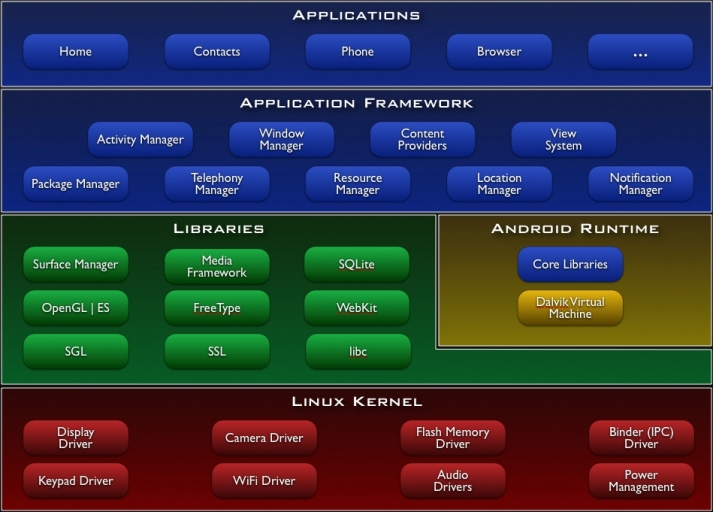
\includegraphics[width=0.7\columnwidth]{figs/system-architecture}
\caption{An overview of the Android system architecture, from \citep{androidarchitectureoverview}}
\label{fig:androidoverview}
\end{center}
\end{figure}


\section{Android Architecture Overview}
Android is an open-source project, built on Linux. Designed to be a lightweight, modular, extendable, and versatile operating system, Android removed almost all of the typical GNU/Linux stack, and wrote an entire framework from scratch. Built in Java, Android runs the Dalivk VM, a lightweight Java-compatible VM (see Figure \ref{fig:androidoverview}). 

The three major application components of Android are Activities, Services, and Content Providers. They are joined together through the Intent system. Activities are user-facing tasks, and follow the iOS definition of an ``app''. Only one may run at a time, and they have strict lifecycles. Services run in the background and follow a less strict lifecycle. Their main purpose is to perform long-running tasks that do not require user input. Lastly, Content Providers ``manage access to a structured set of data. They encapsulate the data, and provide mechanisms for defining data security. Content providers are the standard interface that connects data in one process with code running in another process''\citep{androidcontentproviders}.

Android was built from the ground-up to be composed of strongly isolated modules with little dependencies. No traditional SysV IPC is allowed; instead Android provides its own inter-app communication built off of its Intent system. Intents on Android, as described in the documentation, are ``an abstract description of an operation to be performed... An Intent provides a facility for performing late runtime binding between the code in different applications. Its most significant use is in the launching of activities, where it can be thought of as the glue between activities. It is basically a passive data structure holding an abstract description of an action to be performed''\citep{androidintents}. Intents allow apps to describe the operation they would like to perform, without explicitly identifying a recipient. For example, when the intent \textit{ACTION\_VIEW} is sent with data ``http://google.com'', Android searches through all installed apps that designate that they respond to that intent and will pick one to deliver it to; in this case, the \textit{Browser} would respond.

\section{Android Permissions}
The highly modular and decentralized aspect of Android makes it extremely easy to tap into virtually all Personally Identifiable Information on the device. To protect this, and many other aspects of the system, Android utilizes the Permission security model. The permission security model is a static list of capabilities an app possesses: when presented with this list before installation (see Figure \ref{fig:gpstorepermissions}), a user will either grant the app access to the features or simply not install the app. When an app requests a permission, the Android system treats it as if the user granted the app that capability. After installation, this list will never change unless the app package itself changes and the user reviews the new permissions.

\begin{figure}[h]
\begin{center}
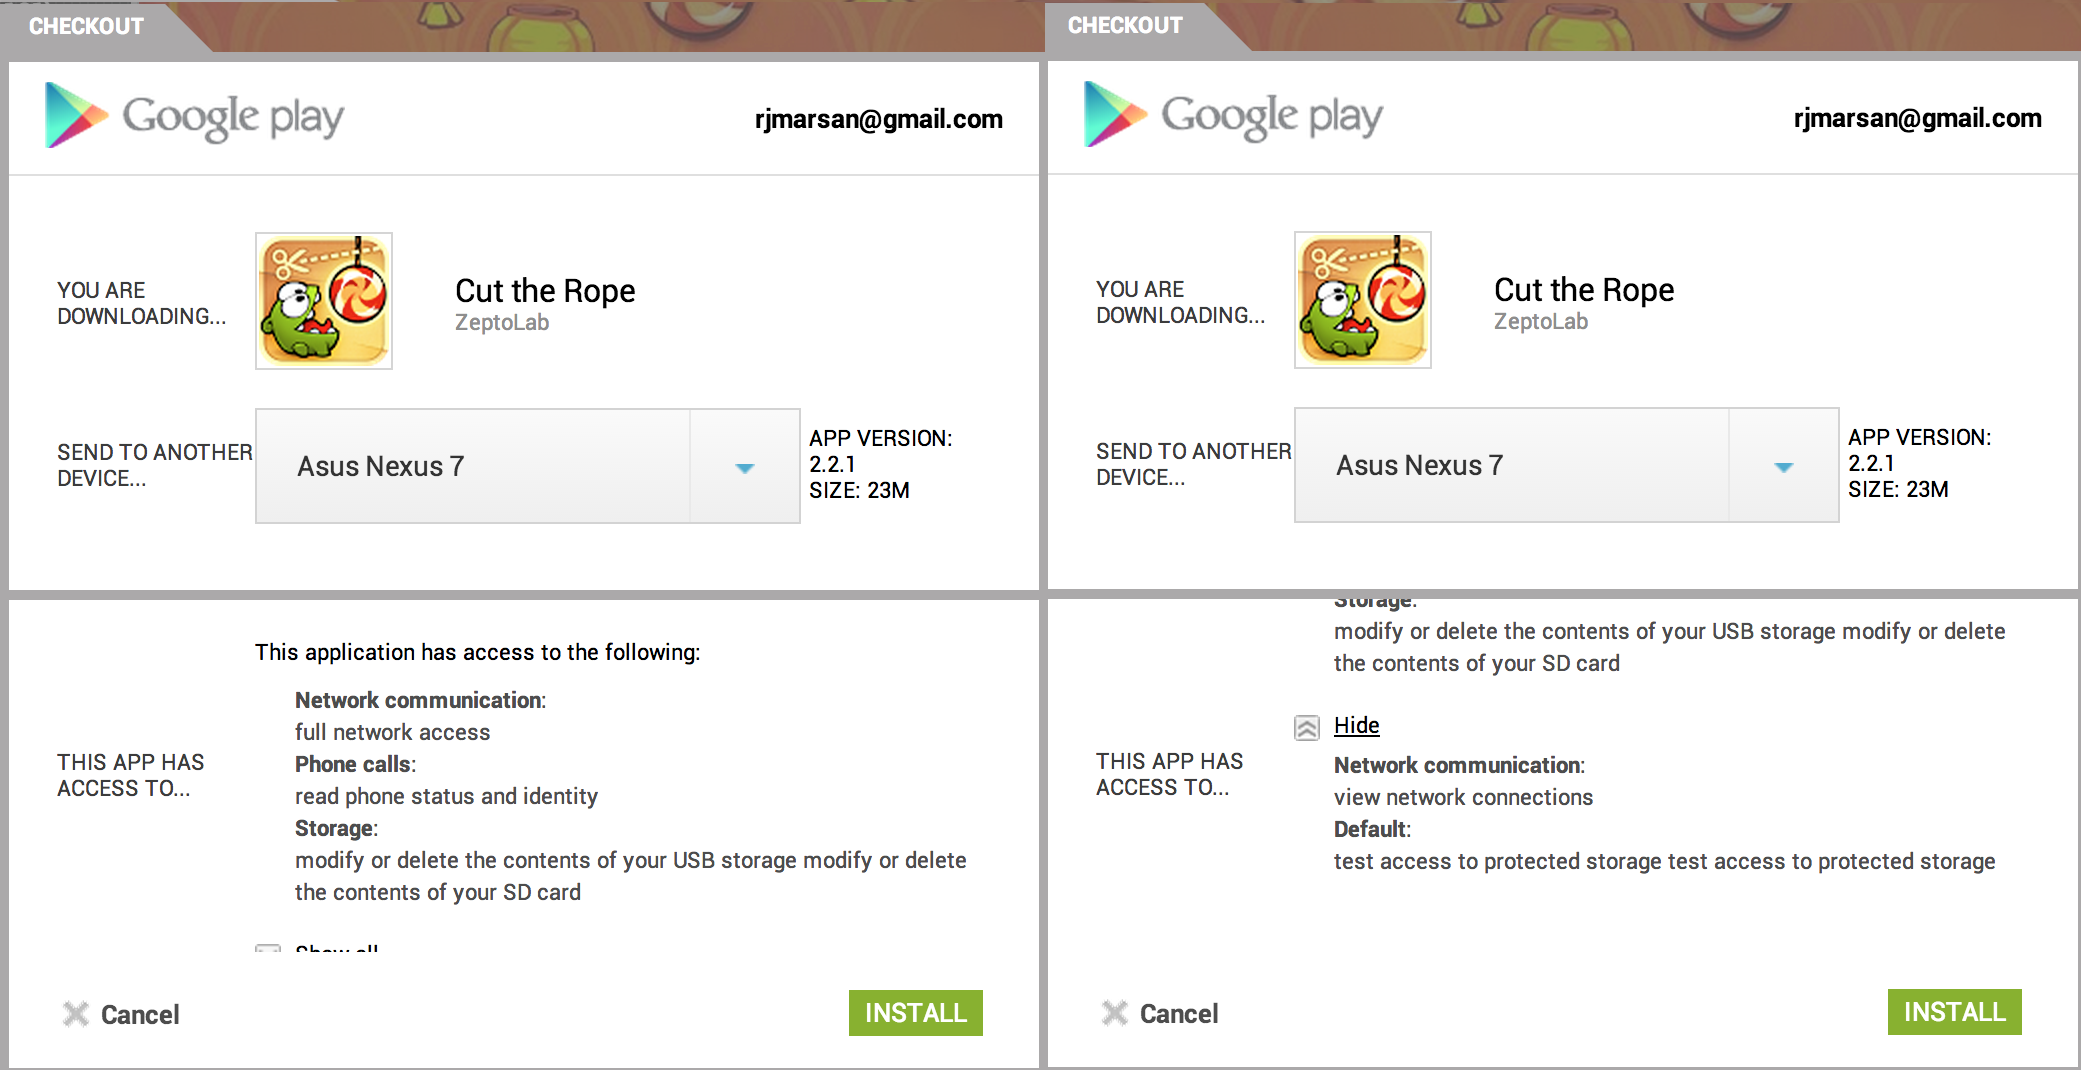
\includegraphics[width=1.0\columnwidth]{figs/GPStoreInstallScreen}
\caption{A sample Google Play Store install screen showing the permissions. The user must scroll to see all of them, and click ``Show All'' to see the hidden ones.}
\label{fig:gpstorepermissions}
\end{center}
\end{figure}

Android permissions themselves are much more granular than a typical UNIX permission system. They cover a wide variety of operations, including controlling the sleep state, accessing hardware, accessing PII, and many system operations. Some of the most requested permissions can be seen in Table \ref{tab:perms}; the rest can be seen in Appendix Table \ref{tab:allperms}.

%\begin{smitemize}
%\item \textit{android.permission.INTERNET}: Grants the app access to network sockets. Without this, an app alone could not access the internet over WiFi, 3G, or other interfaces. No restrictions are placed on the protocol, ports, or domains accessed.
%\item \textit{android.permission.WAKE\_LOCK}: Prevents the device from sleeping. When a Wake Lock is acquired, the Android system will not shut off. Depending the Wake Lock, the screen may continue to stay on, or it may turn off, but the CPU and other hardware remains in operation.
%\item \textit{android.permission.READ\_PHONE\_STATE}: Grants the app access to the phone hardware, which includes IMEI, GSM information, as well as the phone number of the current call. Since the IMEI is frequently used as a UDID, this is a popular permission.
%\item \textit{android.permission.CAMERA}: Allows apps access to the camera hardware, if present. The Android system still requires an app hold a valid drawing surface before data is sent to the app, making it difficult to perform in the background.
%\item \textit{android.permission.READ\_CONTACTS/READ\_SMS/READ\_CALENDAR}: offers read-only access to personal information. <say more?>
%\item \textit{android.permission.WRITE\_CONTACTS/WRITE\_SMS/WRITE\_CALENDAR}: offers write-only access to personal information. <say more?>
%\end{smitemize}





\begin{table*}[t]
\begin{small}
\begin{tabular}{p{3cm}|p{12.5cm}}
Permission  & Description \\
\hline

\textit{INTERNET} & Network communication. full Internet access. Allows the app to create network sockets.  \\
\textit{WRITE\_EXTERNAL\_\-STORAGE} & Storage. modify/delete USB storage contents modify/delete SD card contents. Allows the app to write to the USB storage.  Allows the app to write to the SD card.  \\
\textit{READ\_PHONE\_STATE} & Phone calls. read phone state and identity. Allows the app to access the phone features of the device.  An app with this permission can determine the phone number and serial number of this phone, whether a call is active, the number that call is connected to and the like.  \\
\textit{ACCESS\_FINE\_\-LOCATION} & Your location. fine (GPS) location. Access fine location sources such as the Global Positioning System on the tablet, where available.  Malicious apps may use this to determine where you are, and may consume additional battery power.  \\
\textit{ACCESS\_COARSE\_\-LOCATION} & Your location. coarse (network-based) location. Access coarse location sources such as the cellular network database to determine an approximate tablet location, where available.  Malicious apps may use this to determine approximately where you are. \\
\textit{WAKE\_LOCK} & System tools. prevent tablet from sleeping prevent phone from sleeping. \\
\textit{READ\_CONTACTS} & Your personal information. read contact data. Allows the app to read all of the contact (address) data stored on your tablet.  Malicious apps may use this to send your data to other people. \\
\textit{CALL\_PHONE} & Services that cost you money. directly call phone numbers. Allows the app to call phone numbers without your intervention.  Malicious apps may cause unexpected calls on your phone bill.  Note that this doesn't allow the app to call emergency numbers.  \\
\textit{CAMERA} & Hardware controls. take pictures and videos. Allows the app to take pictures and videos with the camera.  This allows the app at any time to collect images the camera is seeing.  \\
\textit{WRITE\_CONTACTS} & Your personal information. write contact data. Allows the app to modify the contact (address) data stored on your tablet.  Malicious apps may use this to erase or modify your contact data.  \\
\textit{GET\_TASKS} & System tools. retrieve running apps. Allows the app to retrieve information about currently and recently running tasks.  Malicious apps may discover private information about other apps.  \\
%\textit{WRITE\_SETTINGS} & System tools. modify global system settings. Allows the app to modify the system's settings data.  Malicious apps may corrupt your system's configuration.  \\
\textit{RECORD\_AUDIO} & Hardware controls. record audio. Allows the app to access the audio record path.  \\
\textit{SEND\_SMS} & Services that cost you money. send SMS messages. Allows the app to send SMS messages.  Malicious apps may cost you money by sending messages without your confirmation.  \\
\textit{READ\_HISTORY\_\-BOOKMARKS} & Your personal information. read Browser's history and bookmarks. Allows the app to read all the URLs that the Browser has visited, and all of the Browser's bookmarks.  \\
\textit{READ\_CALENDAR} & Your personal information. read calendar events plus confidential information. Allows the app to read all calendar events stored on your tablet, including those of friends or coworkers.  Malicious apps may extract personal information from these calendars without the owners' knowledge. \\
\textit{WRITE\_HISTORY\_\-BOOKMARKS} & Your personal information. write Browser's history and bookmarks. Allows the app to modify the Browser's history or bookmarks stored on your tablet.  Malicious apps may use this to erase or modify your Browser's data \\
\textit{RECEIVE\_SMS} & Your messages. receive SMS. Allows the app to receive and process SMS messages.  Malicious apps may monitor your messages or delete them without showing them to you.  \\
\textit{WRITE\_CALENDAR} & Your personal information. add or modify calendar events and send email to guests without owners' knowledge. Allows the app to send event invitations as the calendar owner and add, remove, change events that you can modify on your device, including those of friends or co-workers.  Malicious apps may send spam emails that appear to come from calendar owners, modify events without the owners' knowledge, or add fake events.  \\
%\textit{CHANGE\_WIFI\_STATE} & System tools. change Wi-Fi state. Allows the app to connect to and disconnect from Wi-Fi access points, and to make changes to configured Wi-Fi networks.  \\
%\textit{ACCESS\_MOCK\_LOCATION} & Your location. mock location sources for testing. Allows the app to create mock location sources for testing.  Malicious apps may use this to override the location and/or status returned by real location sources such as GPS or network providers.  \\
%\textit{PROCESS\_OUTGOING\_CALLS} & Phone calls. intercept outgoing calls. Allows the app to process outgoing calls and change the number to be dialed.  Malicious apps may monitor, redirect, or prevent outgoing calls.  \\
%\textit{MODIFY\_AUDIO\_SETTINGS} & Hardware controls. change your audio settings. Allows the app to modify global audio settings such as volume and routing.  \\
\textit{MOUNT\_UNMOUNT\_\-FILESYSTEMS} & System tools. mount and unmount filesystems. Allows the app to mount and unmount filesystems for removable storage.  \\
\textit{READ\_SMS} & Your messages. read SMS or MMS. Allows the app to read SMS messages stored on your tablet or SIM card.  Malicious apps may read your confidential messages. \\
\textit{READ\_LOGS} & Your personal information. read sensitive log data. Allows the app to read from the system's various log files.  This allows it to discover general information about what you are doing with the tablet, potentially including personal or private information.  \\
\textit{DISABLE\_KEYGUARD} & System tools. disable keylock. Allows the app to disable the keylock and any associated password security.  A legitimate example of this is the phone disabling the keylock when receiving an incoming phone call, then re-enabling the keylock when the call is finished.  \\
%\textit{BLUETOOTH} & Network communication. create Bluetooth connections. Allows the app to view the configuration of the local Bluetooth tablet, and to make and accept connections with paired devices. \\
%\textit{WRITE\_SMS} & Your messages. edit SMS or MMS. Allows the app to write to SMS messages stored on your tablet or SIM card.  Malicious apps may delete your messages. \\
%\textit{CHANGE\_CONFIGURATION} & System tools. change your UI settings. Allows the app to change the current configuration, such as the locale or overall font size.  \\

\end{tabular}
\end{small}
%\vspace{-0.2in}
\caption{Frequently Requested Android permissions, and the GPStore's description of them}
\label{tab:perms}
%\vspace{-0.1in}
\end{table*}





In cases like \textit{WAKE\_LOCK} and \textit{CAMERA}, the permission seems fairly singular: access to exactly one feature. However, for other permissions, such as \textit{INTERNET} and \textit{READ\_PHONE\_STATE}, many more granularities could be established. For example, \textit{INTERNET} gives unconditional access to all domains, unlike web pages in modern web browsers. In addition, while permissions are intended to be non-overlapping, there still are ways --- varying from minor to major --- to acquire information guarded by one permission from another. For example, \textit{READ\_PHONE\_STATE} can access to the current phone call, and is able to establish call logs, an operation normally protected by \textit{READ\_CONTACTS}. There are some permissions, however, that are explicitly supersets of another other, such as \textit{ACCESS\_COURSE\_LOCATION} --- providing network-tower location --- and its superset, \textit{ACCESS\_FINE\_LOCATION} --- providing GPS location. 

Permissions do not tend to change through Android's release history. As new hardware is made accessible through Android's SDK, new permissions are added for them, but there are very few times when permissions drastically change meaning or scope. Through Android's 6 year history, only 3 new permissions has been added to restrict previously unrestricted operations\footnote{In Android 4.1, the storage device requires a permission to read, and the call logs require a separate permission to read and write --- previously they shared a permission with contacts\citep{android41new}.}.

\section{Permission Enforcement}
Permission enforcement on Android is generally performed in two main ways: UNIX permissions and explicit runtime checking. Most hardware is accessible using C or other low-level calls, so permissions are more effectively enforced via UNIX Group Permissions. Upon app installation, Android assigns each app a unique UID and assigns different group permissions to that user. For example, socket access is granted to a UNIX group, and all apps that request \textit{INTERNET} are added to that group. This is simple, effective, and has very little performance overhead. Unfortunately, it makes it difficult to put any additional enforcements as to when and how these resources are accessed. 

System operations, like wake locks, changing system settings, turning on and off components, is checked on every API call, through a centralized PackageManager class. The PackageManager first checks if the app has requested that permission. If it has, it then proceeds to check if the permission is protected by the system. Some permissions are only available to trusted code, through either a shared key, or being located in a system folder. Many system operations fall into this category, including \textit{WIPE\_DEVICE}, and \textit{BRICK}. These operations typically are extremely dangerous, and have the potential to destroy a device, or perform elaborate phishing operations. Even if an app requests the permission, the PackageManager still has the right to reject the operation. This allows system-level operations to be exposed to trusted developers post-deployment on a device, while still protecting the operations from untrusted developers.

The final aspect of permissions deal with protecting PII. Android implements the bulk of PII sources through Content Providers, which sit in front of a dataset and provide access to remote services. It is therefore imperative for each individual data source to check the permissions of the incoming app, every time it is requested. This, however, provides opportunities to extend on its behavior.

\subsection{Permission Rejection}
\label{sec:permissionrejection}
When a permission is checked on Android, one of two outcomes is possible. The check passes, and the operation continues as intended, or the check fails, and an exception is thrown. By design, the code path instantly jumps to an error state, halting the action. No logging of this action takes place, nor are partial passes allowed.

\section{Third Party Permissions}
\begin{sloppypar}
Android was built to distribute PII in a modular fashion, and it extended these features to other third party apps. Any developer may write Content Providers, and likewise, can create Permissions to protect them. Other apps must request that permission before accessing the data. An example of this: Alice writes a messaging app, \textit{MyMessenger}. She wants to expose the PII to other apps, so she makes a Content Provider around it. To protect the user's information, she defines her own permissions: \textit{mypackage.MyMessenger.READ\_MESSAGES} and \textit{mypackage.MyMessenger.WRITE\_MESSAGES}. Bob writes an app that uses \textit{MyMessenger}'s data to build a picture. His app requests the permission \textit{mypackage.MyMessenger.READ\_MESSAGES}. When his app contacts Alice's Content Provider, she checks this custom permission before proceeding with the query. However, if Bob does not request \textit{mypackage.MyMessenger.WRITE\_MESSAGES} and attempts to perform a write action, Alice's Content Provider will reject the operation.
\end{sloppypar}
%These rejections are not logged or notified. expand on this.


If two apps request the same permissions, as long as neither have access to system permissions, it can be assumed that they have the same capabilities. These capabilities are permanent as well, as permissions for a given package can not be added nor removed. This Permission Fingerprint, or set of capabilities, uniquely defines what an app has access to. All apps that request the same set of permissions have access to the exact same set of actions, and only through those permissions do they have those actions (with a few exceptions). However, Android permissions are static, therefore a Permission Fingerprint doesn't guarantee a specific pattern of behavior. In fact, since not all permissions are guaranteed to be granted, a Permission Fingerprint simply establishes the absolute maximum capabilities of an app - even if the system rejects some of them.

\chapter{Malware on Android}
\label{sec:malware}

Malware on mobile devices has seen a departure from past exploits. The wealth of Personally Identifiable Information easily available on mobile OSs increasingly makes them the focus of malicious software. In addition, the tight sandboxing constraints often forces malware writers to either find exploits to break out of the sandbox or to write malware that cloaks itself as benign. Without finding exploits, code can not be run by the user unless it is in it is form and comes through a trusted channel (unless of course that security feature has been disabled). Once on the device, malware has several main methods of attack.

\section{Installation}
The three primary ways in which malware can be installed on an Android device are \textit{Repackaging}, \textit{Update Attack}, and \textit{Drive-by Download}\citep{zhou2012dissecting}. The first two are designed to sneak malware into the Google Play Store or other third party stores; and the third is designed to trick the user into installing it by mistake. \textit{Repackaging} deals with the technique of taking an existing app, adding malicious code to it, and repackaging it again (discussed further in Chapter \ref{sec:incognitoware}). \textit{Update Attacks} typically build off of \textit{Repackaging}, but do not acquire malicious code until later, making static detection difficult\citep{zhou2012dissecting}. The last, \textit{Drive-By Downloads}, is often tied with \textit{Repackaging}, but is not presented in an official app channel. Instead, it is downloaded when the user visits a webpage or clicks a link\citep{zhou2012dissecting} and Android prompts the user as to whether or not they would like to install the app. All three methods involve concealing the intent of the malware and passing as a legitimate app; they do not use browser exploits or system exploits to install the initial malware without the user's consent.

\section{Malicious Actions}
Once installed on the device, Android malware has several main methods of attack. Xuxian Jiang
 and Yajin Zhou\citep{zhou2012dissecting}, along with Spreitzenbarth\citep{spreitzenbarth2013}, and Hackmageddon\citep{hackmageddon2011} define four major categories: \textit{Privilege Escalation Attack}, \textit{Remote Control Attack}, \textit{Monetary Service Attacks}, and \textit{Privacy Info Theft}. 


\section{Privilege Escalation Attack}
\textit{Privilege escalation attacks} take several forms on Android. The basic premise is simple: acquire access to operations beyond what the sandbox and granted capabilities provide. The main way to accomplish this is via \textit{rooting}.

\subsection{Rooting}
\textit{Rooting} is the act of acquiring root --- or administrative privileges --- on an OS. Typically mobile OSs do not provide the user or apps with root capabilities and instead reserve that for a set of trusted system processes. However, by finding vulnerabilities in these services or exploiting the OS itself, apps can escape the sandbox. After an app has been granted root capabilities, the permission system no longer applies to it: it can simply access whatever it wants. These attacks are difficult for the system to detect as all monitoring of apps relies on monitoring the sandbox --- there is no way to track an app that escapes the sandbox. This technique is commonly employed by botnets, giving remote access to the core system. 

Many examples of root exploits exist, dating back to 2011 with \textit{RageAgainstTheCage}\citep{droiddream}. These root exploits were very popular for non-malicious purposes, circumventing the device's sandbox to install a permanent root binary, creating a similar setup to a typical UNIX computer, where root may be acquired after a password and/or permission. In March 2011, however, DroidDream was discovered. DroidDream used \textit{RageAgainstTheCage} to silently install additional applications in the background, stealing PII and forming a botnet. By the time Google remotely removed it from the market, it had been downloaded an estimated 50,000 to 200,000 times\citep{castillo2010android}, which was the largest bulk-remote-removal of apps seen from the GPStore. From then on, a stream of root exploit malware was found based off of exploits such as \textit{RageAgainstTheCage}, \textit{udev}, and another called \textit{GingerMaster}\citep{gingermaster}.

\subsubsection{Recent Android Rootkits}
\label{sec:recentrootkits}
\textit{GingerMaster}\citep{cskills2011} is significant because it is the last known root exploit malware seen in use. Designed for Android 2.3.3, it can currently run on 45\% of all Android devices in use, according to the official Android Dashboard\citep{androiddashboard}. In reality, however, of that 45\%, almost all have been patched to fix the exploit\citep{cskills2011}. All previous exploits were patched in Android 2.3\citep{cskills2011}, meaning less than 6\% of all active Android devices are vulnerable to them. Since Android 4.0, Google has focused greatly on security, improving ASLR\citep{threatpost2012} and hardening system services\citep{androidjbsecurity}. No known rootkits exist --- malicious or not --- for Android 4.0 and up comprising 54\% of active Android devices.

 %Several exploits became very popular for malware writers, starting with DroidDream in 2010 <cite>, then RageAgainstTheCage, PSNeuter, and GingerBreak. When DroidDream was first discovered, it was downloaded over <50,000> times in the GPStore - prompting the largest bulk-remote-removal of apps Google has ever been discovered to have performed. However, most of these attacks have been fixed by vendors as of Android 2.3.3 - meaning the total amount of current devices in use that are vulnerable to these bugs being roughly <10%>. After these attacks, Android has taken definite steps to up its security. Since 4.0, proper ASLR has been implemented, as well as other security enhancements. There has been no known malware written for Android 4.0 and up - over <50%> of the active market.

\subsection{Confused Deputy Attack}
The second main vector for privilege escalation attacks is the \textit{confused deputy attack}\citep{hardy1988confused}. In this scenario, services that guard sensitive operations are ``tricked'' into performing them. For example, if a Content Provider forgets to check a permission, or if a developer finds APIs that do not correctly perform a permission check. Perhaps the simplest example of this is the ability for any Android app to contact remote servers by asking the web browser to open a URL. By including sensitive data in the URL, an app may still transmit sensitive data to a remote server without ever requesting the \textit{INTERNET} permission. Projects like XManDroid\citep{bugiel2011xmandroid} and Quire\citep{dietz2011quire} address this by extending Android to analyze inter-app communication and detect this kind of attack. %Despite all of these concerns, it is worth noting that no known malware has been used to exploit this. 

\section{Remote Control Attack}
\textit{Remote Control Attacks}, frequently called \textit{botnets}, are the ability for malware to accept commands from a remote server, controlling the device. This technique is common --- Xuxian Jiang
 and Yajin Zhou\citep{zhou2012dissecting} found in 93\% of Android malware --- and is often used in conjunction with other attacks\citep{spreitzenbarth2013}.

\section{Monetary Service Attack}
\label{sec:premiumsms}
The second malware technique is possibly the simplest: perform services on behalf of the user that cost money. Examples of this include calling costly phone numbers and sending premium SMS messages. Typically these actions are performed without notifying the user, and are only visible after the user checks their bill. These attacks have been prevalent in the Android market for quite a while, with NQ Mobile\citep{nq2013} listing it as one of the top three threats of 2012, and being found in 39 of 119 of the malware documented by Spreitzenbarth\citep{spreitzenbarth2013}. However, recent versions of Android (after 4.2 Jelly Bean\citep{androidjbsecurity}) have taken the step of warning the user before premium SMSs are sent. %This attack vector, while common, will see a reduction in the future thanks to these measures.

A prime example of this is FakeInst\citep{avastfakeinst}, a repackaged version of Instagram\citep{instagramandroid} that sent premium SMS messages on start. ``In the background, the fake downloader sends a premium rate SMS to the number based on the country of origin for the user''\citep{avastfakeinst}. In many cases, the premium SMS messages would end up being billed to the user for over \$4 each\citep{avastfakeinst}, without ever alerting the user. Messages are often deleted by the app, removing the trace until the user gets their bill.
%\temp{Expand on this more}
%show some examples of this. expand on this more.

\section{Private Info Theft}
The last malware technique is the most significant, and represents the largest departure from typical malware: apps that steal PII, or \textit{Info Theft Malware}. The theme is fairly straightforward: provide the user with a seemingly legitimate app, but in the background acquire large amounts of valuable data --- including call logs, contacts, and photos --- and send them to a remote server. This fits with the main themes of mobile computing: the consolidation of many sources of PII all in one device. 
%However, this is the biggest departure from typical malware. 
To the system no unusual operations are performed and no exploits are ran. The qualification for Info Theft Malware lies in the ``use'' vs ``misuse'' of PII; often times, this line is blurred.

\subsection{Path on iOS}
\label{sec:path}
A large distinction of what constitutes as privacy malware to an individual stems from the user's expectations of how the app will use their PII. Consider the case of the Path iPhone app, which in February 2012 was discovered to be uploading the user's entire contact list to Path's servers, without any consent from the user\citep{thampi2012}. It is fairly uncontroversial for a social network to read your contact data, and the act of scanning contacts to help ``find your friends'' on Path wasn't out of the ordinary. As VentureBeat discovered: ``Facebook, Twitter, Instagram, Foursquare, Foodspotting, Yelp, and Gowalla are among a smattering of iOS applications that have been sending the actual names, email addresses and/or phone numbers from your device's internal address book to their servers''\citep{vb2012addressbook}. Ultimately, however, the outrage was sparked because of how unexpected the behavior was.

The Path incident sparked several key changes in iOS's security model: having a popup occur when an app requests access to the contacts database and allowing the user to reject the request. This, in general, is a one-time request, after which the app is granted unrestricted access to the content\citep{AppleContacts}. This change, however, did not fully address situations like Path, in which is was less about the app simply having access to the data, and more about what the app actually did with the data behind the scenes. When these actions did not match up with user expectations, it was treated as malware until the situation was cleared up by Path. The next day, they issued an update immediately explaining to the user what they were going to do with the data, and why.

It is worth noting that the only reason Path's contacts upload mechanism was discovered was by accident: Arun Thampi discovered it as part of a company hackathon, and only via sniffing the HTTP requests coming from the phone. An ordinary smartphone user would not have access to these tools, nor have the time and patience to sift through the data to spot unusual behavior. These actions are unchecked and hidden from the user, not giving them a chance to decide for themselves if they are comfortable with them - supporting our motivation for AndroMEDA.

\section{User-App Agreement}
This incident, however, lies at the heart of mobile malware: Misuse of PII lies in the abstract definition of how the app is expected to behave. Apps that violate this expectation of behavior are classified as malware, and apps that do not are not. This agreement between the user and the app, the User-App Agreement (or UAA), is an informal understanding the user has as to what actions an app will take. This differs from the Permission Fingerprint, which is a measure of what actions the app is capable of performing, instead dealing with exactly when and how those actions are taken. Since this agreement is not formally defined, it is acquired through external trust in an app. This happens in various ways, through the description the app provides, to the knowledge and referral of the app from other trusted sources, or the trust in the developer. The UAA is not a measure of how trustworthy an app is, but rather a framework for the user consenting and trusting specific actions an app may take.

\subsection{UAA Example - Social Networking App}
An example of UAA can be seen in the expected behavior of a hypothetical app and user. The first is a large Social Networking app, which requests permission to access internet, send SMS messages and read the contacts database. If the Social Networking app accesses contacts when the user requests it ``find my friends'', and it sends SMS messages after the user messages another user who is not ``online'', these actions fall within the UAA of the Social Networking app and the user. However, if the contacts database is read and uploaded to a remote server without the consent of the user, this may violate the UAA, breaking the trust of the user (building off the example of Path). 

\subsection{UAA Example - Social Game}
The other example is a little known developer's game, which also requests permission to access internet, send SMS messages and read contacts, same as the Social Networking app. These documented capabilities in the Permission Fingerprint may be enough to violate the UAA: the user may not trust an app with the capability of these actions. However, in the case that the user does, or simply doesn't pay attention, the app still may not violate the UAA. If the app is an online game, and asks you to find other people you know who are playing it, this would more likely than not violate the UAA. However, if it sends SMS messages to your friends telling them to download the game, this would breech the UAA, breaking the trust of the user.

In both examples, the apps have the exact same Permission Fingerprint, but vary wildly in their expected behavior, and which actions are trusted and untrusted. This fits right along with our definition of malware, with the misuse of PII and other device capabilities. This also highlights the shortcomings of the Permissions framework - being unable to deal with the subtle differences between trusted behavior and untrusted behavior. Indeed, for any given user, they may have a very different understanding of what acceptable behavior is. Therefore, UAA plays a crucial role in classifying apps in relation to Info Theft Malware.

\section{Proof of Concept Malware in Academia}
In the realm of malware research in academia, several prominent proof-of-concept examples further demonstrate the vague line between use and misuse of PII, and our concept, the User-App Agreement. The most notable one is SoundComber\citep{schlegel2011soundcomber} It passes off as a benign app, but in the background records audio, and does on-phone processing to find sensitive PII, after which it uploads the information to a remote server. This app is unique because of its simple Permission Fingerprint, and its ability to gather sensitive PII from a channel not suspected to be very rich in PII.

The second prominent example of academic malware on Android is TapLogger\citep{xu2012taplogger}. TapLogger imitates a simple touch-based game, learning the vibration patterns of the device for each tap. After which, TapLogger records the vibration patterns in the background, attempting to discover passwords and other sensitive keyboard events, all through a seemingly trusted sensor. TapLogger requests no Permissions, therefore its behavior is a possible behavior of virtually all apps. 

In Chapter \ref{sec:incognitoware}, we build upon these examples to present an additional dataset of research IncognitoWare, or repackaged apps with malicious software added. We keep the Permission Fingerprints identical to the cloned app, making detection exceptionally difficult. 
%reference future malware set

\section{Conclusion}
The landscape of malware on Android follows many clear patterns. The first is the use of masquerading as benign apps, and passing through trusted/semi-trusted channels to enter the device. Once on the device, the four main categories of attacks are privilege escalation attacks, remote control attacks, monetary service attacks, and info theft. Of these three attacks, privilege escalation and monetary service attacks are the easiest to protect against, and indeed Android has taken serious steps to mitigate these. However, the third time of attack, Info theft, is the most difficult to mitigate on Android, due to the shortcomings of the Permissions framework, and the wide spectrum of severity these attacks can take. Since these attacks may vary in interpretation per user, and lay in the subtle communication between the user and the app, we highlight the need for a concise representation UAA, where the user can evaluate the actions themselves.

\chapter{Conclusion and Future Work}
\label{sec:conclusion}
\section{Conclusion}
AndroMEDA helps users understand the context in which their Personally Identifiable Information is used, which allows them to make more informed decisions on whether an app is action maliciously or not. 

In this paper, we introduced 3 key items:
\subsection{User-App Agreement}
%We analyze the state of Android and Permissions, and conclude the need to address the User-App Agreement, which is a framework for consenting and trusting specific actions an app may take. It lies at the heart of classifying Info Theft Malware. Android Permissions address the capabilities of an app, but fail to address the context and use of those capabilities, which are cruicial to trusting an app's actions.

We analyzed the current Android security framework: The Permission System, and found it's main flaws were it's lack of addressing context and use, which we generalize into the User-App Agreement - a framework for consenting and trusting specific actions an app may take. Whereas Android Permissions exceeded at defining general capabilities of an app, and these capabilities go a long way in shaping the User-App Agreement, they fail at addressing the context in which the permissions are used, and what they are used for.

\subsection{\temp{AndroidMarketDB}}
To perform a full analysis of the current state of Android Permissions, we use a novel dataset, \temp{AndroidMarketDB}. By analyzing more than 80\% of apps in the Google Play Store, we are able to better understand the interrelationship of permissions and expected behavior. We produce key insights as to the popularity of apps vs their PII permissions, and when apps deviate from their expected behavior - potentially violating the User-App Agreement. We then analyze a comprehensive malware dataset using the same techniques, and find that many types of malware can be identified purely by it's permission fingerprint. We conclusively show the connection between Permissions and Expected Behavior are present, but not strong enough to differentiate between Info Theft Malware and many popular apps.

\subsection{AndroMEDA}
Building off the concept of the User-App Agreement, we introduce AndroMEDA. Key parts of the User-App Agreement were previously unnoticable to the user until AndroMEDA. By giving the user more information on the context and use of permissions, they can evaluate whether they trust those actions, and ultimately whether the app is acting maliciously or not. This, in turn, helps mitigate Info Theft Malware on Android.

\section{Future Work}
\label{sec:futurework}
AndroMEDA is, ultimately, not a silver bullet at detecting all Android malware. Projects like TaintDroid and TISSA provide functionality that would greatly enhance the abilities of AndroMEDA to visualize context and use of permissions to the user, and allow them to take action against it. 

AndroMEDA could also benefit greatly from the probablistic modeling of pBMDs and Crowdroid, in correlating user action with permission behavior. These would not replace the need to alert the user, but rather be able to better dictate when to put different classes of alerts to the user, as ultimately the decision of what is malware is up to them.

The weath of data in \temp{AndroidMarketDB} was also not fully explored. We are currently interested in seeing if specific keywords in user reviews correlate with malicious software, or other problematic apps. Many more areas of metadata, like the description, developer, etc, can be further explored, to see if it gives additional insight into the nature of malware on Android.

\appendix*

%\include{Appendix.tex}

\backmatter

\bibliographystyle{abbrvnat}
%\bibliographystyle{latex8}
\bibliography{ref}

\end{document}
\endinput
%% End of file `thesis-ex.tex'.
